\section{Verbesserung der Augen}
\label{verbesserung_ElSe}
Zusätzlich zu den 64 Landmarks, die ein Gesicht beschreiben, kann von OpenFace weitere 28 Landmarks für ein Auge bestimmt werden, aus denen dann die Blickrichtung ermittelt wird.\\
Um die Position der Landmarks zu verbessern, kann auf dem Bildausschnitt der Augen der ElSe-Algotithmus eingesetzt werden. Dieser Algorithmus arbeitet auf einem Farbbild um so die Umrisse der Pupille zu berechnen.\\
Da unter den 28 Landmarks die Umrisse von Pupille und Iris beschreiben wird, müssen diese aus dem Ergebnis von ElSe abgeleitet werden. Dabei hat sich eine Veränderung des Radius mit ?? für Pupille und ?? für die Iris bewährt.\\
Allerdings muss das Auge für die Berechnung aus entsprechend vielen Pixeln bestehen, wodurch es im Originalbild mindestens mit 10 Pixeln dargestellt wird, um sinnvolle Ergebnisse zu erhalten. Da diese Berechnung unabhängig der Landmarks ausgeführt wird, empfiehlt sich das Ergebnis zu überprüfen, damit die bestimmte Ellipse auch innerhalb der Augenhöhle liegt.\\
Dabei wird jedes Auge unabhängig vom anderen betrachtet, wodurch sich verschiedene Blickrichtung ergeben. Ab einer Distanz von mehr als ??cm kann die Blickrichtung beider Augen als parallel angesehen und kann entsprechend behandelt werden. Eine Verbesserung ergibt sich, wenn beide Augen anhängig von einander bestimmt werden, damit sich der Fehler minimiert.
\subsection{Farb- nach Grau-Bild - To Do}
Bilder einfügen für jedes Verfahren\\\\
Da die Berechnungen von ElSe auf Grau-Bildern arbeitet, das Eingabebild in Farbe ist, muss es in ein Grau-Bild umgewandelt werden. Dabei soll vor allem der Farbunterschied zwischen Pupille und der Umgebung maximal sein.\\
Um die Auswirkung der verschiedenen Farb- nach Grau-Bilder Konverter zu  ermitteln wurden einige Verfahren verwendet um ihre Auswirkung auf die Detektion zu ermitteln. Nach der Umwandlung von Farb- nach Grauwert wird für die Anwendung das Graubild noch normiert, damit Mindestens ein schwarzes und ein weißes Pixel vorhanden ist.
\subsubsection{Luminance}
Dies ist ein lineares Verfahren, das der menschlichen Farbwahrnehmung entspricht. Eine Gammakorrektur wird bei der Umwandlung nicht verwendet.
\[G_{Luminance} = 0.299 \cdot R + 0.587 \cdot G + 0.114 \cdot B\]
\subsubsection{Gleam}
Bei dem Gleam Verfahren wird jede Farbe (Rot,Gelb und Grün) gleich stark bewertet allerdings wird jeder Farbwert mittels einer Gamma-Korrektur verbessert.
\[G_{Gleam}=\dfrac{R^{\frac{1}{2.2}} + G^{\frac{1}{2.2}} + B^{\frac{1}{2.2}}}{3}\]
\subsection{Gleam New}
Dies ist eine verbesserte Variante von Gleam bei dem zuerst das gesamte Bild Analysiert wird um die Parameter für die jeweilige Gamme-Korrektur zu ermitteln.
\[G_{Gleam New}=\dfrac{R^{r} + G^{g} + B^{bx}}{3}\]
Wobei gilt $\{r,g,b\} = \frac{\log(V_{\max})}{\log(\{R,G,B\}_{\max})}$ mit $V_{\max}$ als maximal möglicher Farbwert und $R_{\max}$ als maximal Vorhandener Rot-Farbwert, $G_{\max}$ und $B_{\max}$ äquivalent.
\subsection{Auswirkung der verschiedenen Verfahren - To Do}
Grafiken neu machen\\\\
Um die einzelnen Verfahren besser Vergleichen zu können wurden Künstliche Augen aus dem Datensatz \cite{database_Eye} verwendet, da die Exakte Position der einzelnen Landmarks bekannt sind.
Da auch in der späteren Anwendung der Augenbereich genauer bestimmt ist, bevor ElSe zum Einsatz kommt wurde, nur der Bildbereich in dem alle Landmarks der Augenlider liegen, somit sind die Bilder etwa 64 auf 29 Pixel groß. Um die Qualität der Berechnung bei verschiedenen Größen zu simulieren, wurde das Bild um den angegebenen Faktor verkleinert.\\
\begin{figure}
	\centering
	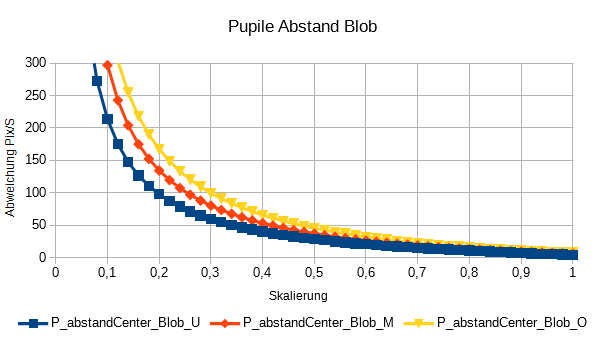
\includegraphics[width=0.45\linewidth]{ElSe_Img/ElSe_22G_Pupile_Zentrum}
	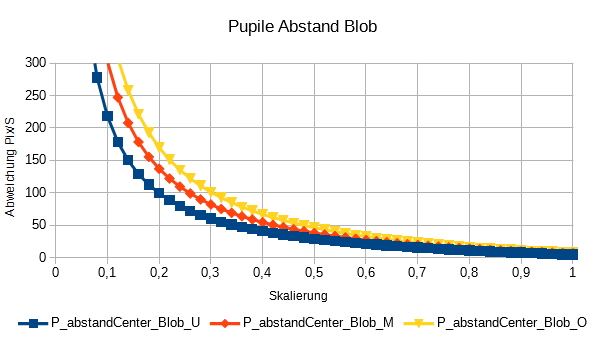
\includegraphics[width=0.45\linewidth]{ElSe_Img/ElSe_Gray_15_Pupile_Zentrum}
	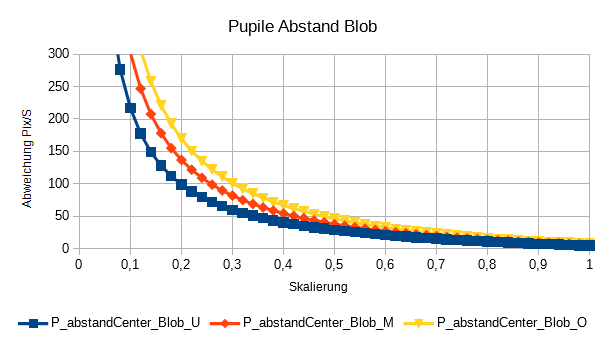
\includegraphics[width=0.45\linewidth]{ElSe_Img/ElSe_Norm_15_Pupile_Zentrum}
	\caption{Abstand des Zentrums der Landmark-Pupille und der Berechneten Ellipse in [Pixel/Skalierung] Oben-Links: Gleam, Oben-Rechts: Gleam New, Unten-Links: Luminance}
	\label{ElSe_Gray_Zentrum}
\end{figure}
\begin{figure}
	\centering
	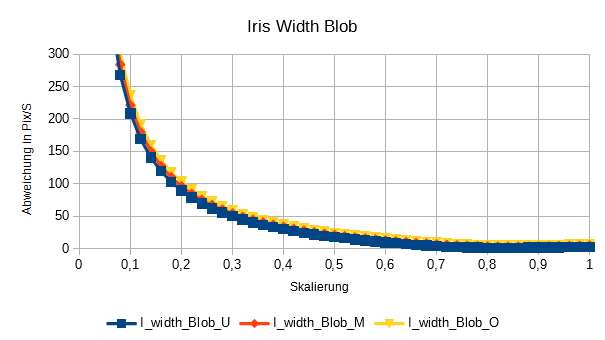
\includegraphics[width=0.45\linewidth]{ElSe_Img/ElSe_22G_Iris_Width}
	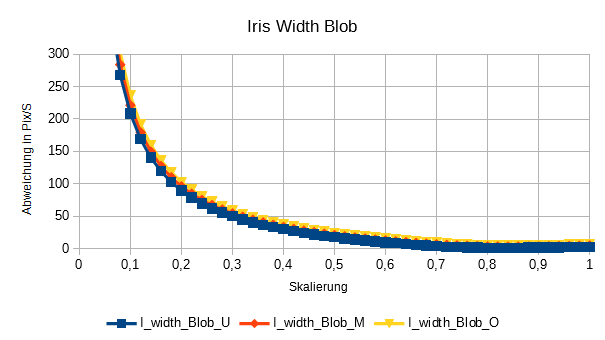
\includegraphics[width=0.45\linewidth]{ElSe_Img/ElSe_Gray_15_Iris_Width}
	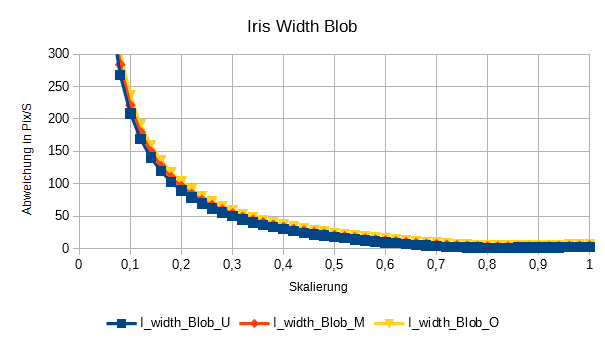
\includegraphics[width=0.45\linewidth]{ElSe_Img/ElSe_Norm_15_Iris_Width}
	\caption{Unterschied Zwischen den Radien der Landmark-Iris und der Berechneten Ellipse in [Pixel/Skalierung] Oben-Links: Gleam, Oben-Rechts: Gleam New, Unten-Links: Luminance}
	\label{ElSe_Gray_Width}
\end{figure}
Es Zeigt sich, dass das Verfahren um den Farbwert in einen Grauwert zu überführen keinen signifikanten Unterschied existiert. Die Differenz zwischen dem besten und schlechtesten Verfahren liegen bei hundertstel Pixel und bei seiner Verkleinerung auf 0.02 auf 1 Pixel unterschied, dies ist so gering, dass das Verfahren Offensichtlich keine Auswirkung auf die eigentliche Berechnung hat.
\subsection{ElSe - Auswirkung des Radius - To Do}
Neu Berechnen ohne Vergrößerung\\\\
Ein weiter wichtiger Parameter des ElSe-Verfahrens ist der Radius des Filters. Wiederrum wurde der Augen-Datensatz \cite{database_Eye} verwendet und diesmal auf der Originalgröße gearbeitet.\\
Im Datensatz besitzen die abgebildeten Augen eine Durchschnittlich Pupille von 15 Pixel und eine Iris von 34 Pixel, wiederum auf dem Bildausschnitt gerechnet.
\begin{figure}
	\centering
	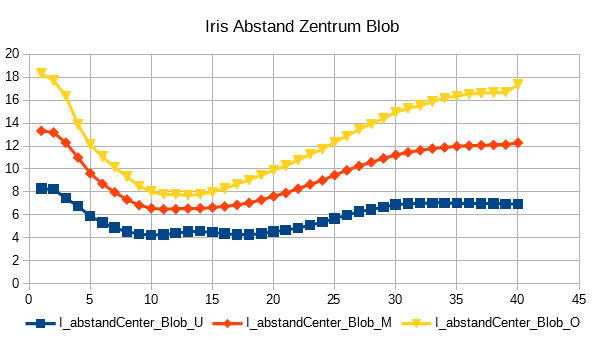
\includegraphics[width=0.45\linewidth]{ElSe_Img/Gray_Alt_Abst}
	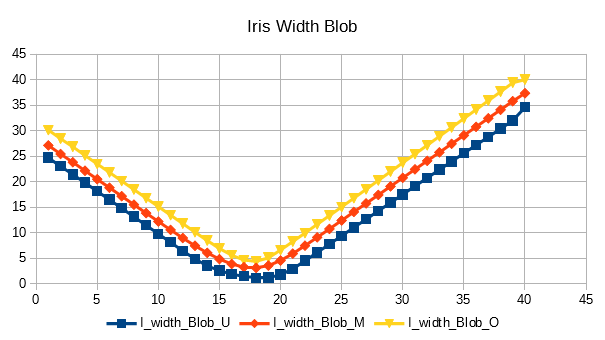
\includegraphics[width=0.45\linewidth]{ElSe_Img/Gray_Alt_Wid}
	\caption{Auswirkung bei der Veränderung des Radius des ElSe-Algorithmus}
	\label{ElSE_Radius}
\end{figure}
Es ist zu erkennen, dass die Wahl des Radius signifikant ist für die Qualität der Berechnung. Im Versuch hat sich ein Radius von etwa einem Zehntel des zu erwartetem Durchmesser der Iris als sinnvoll erwiesen, um möglichst genaue Ergebnisse zu erhalten. Dabei ist zu erwähnen das eine Differenzierung zwischen Iris und Pupille meist nicht möglich ist, da der Grauwert meist recht gering ist und deutlich weniger als der Grauwert vom Rest des Auges.\\
Die Korrekte Größe der Pupille bzw. Iris wird nur mäßig gut ermittelt, da meist eine Zwischenlösung beider berechnet wird und danke der Ruflektionen und Augenfarben nicht klar getrennt werden. Betrachtet man den ermittelten Abstand, siehe \autoref{ElSe_Gray_Zentrum}, sieht man, dass dieser recht konstant bleibt, somit ist dieses Verfahren recht stabil gegenüber Skalierung und wird selbst bei verschiedenen Radien noch gut ermittelt.
\subsection{OpenFace - Auge To Do}
Als Referenz wir das Ergebnis von OpenFace für die zusätzlich bestimmten Landmarks der Augen verwendet. Dies wurde auch auf dem Augendatensatz \cite{database_Eye} angewendet um vergleichbare Ergebnisse zu erhalten.
\begin{figure}
	\centering
	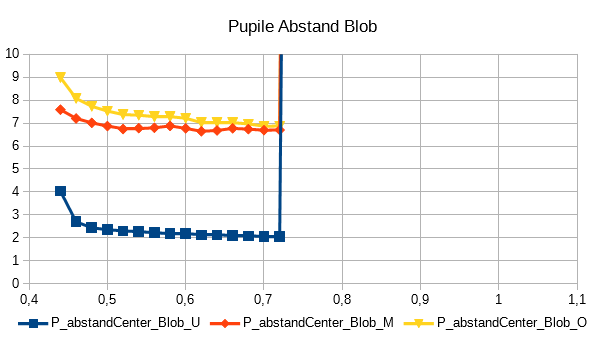
\includegraphics[width=0.45\linewidth]{ElSe_Img/OpenFace_Pupile_Abstand}
	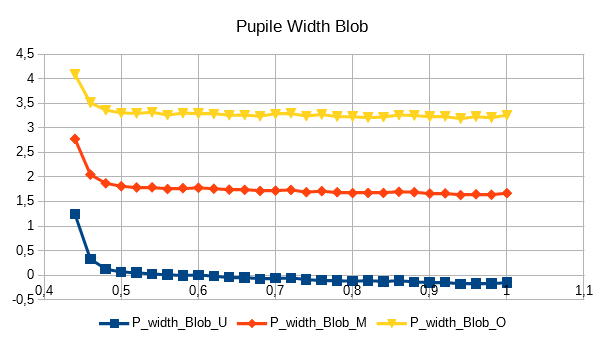
\includegraphics[width=0.45\linewidth]{ElSe_Img/OpenFace_Pupile_Width}
	\caption{}
	\label{OpenFace_Eye}
\end{figure}
Es ist zu erkennen dass dieses Verfahren oft schlechtere Ergebnisse liefert als das Ergebnis von ElSe, allerdings ohne das begehen von großen Fehlern und auch öfters genauere Ergebnisse.\\
\begin{itemize}
	\item Grafik neu
	\item Vergleich zu ElSe
\end{itemize}

